\documentclass[border=10pt]{standalone}
\usepackage{amsmath,amssymb}
\usepackage{tikz}
\usetikzlibrary{arrows.meta,positioning,calc,shapes.geometric,fit,backgrounds,chains}
\usepackage{xcolor}

% ---- palette --------------------------------------------------------------
\definecolor{enc}{HTML}{4A78B0}
\definecolor{add}{HTML}{7A5AA0}
\definecolor{proj}{HTML}{B05454}
\definecolor{vio}{HTML}{B89020}
\definecolor{lens}{HTML}{5A9555}
\definecolor{target}{HTML}{6B7A8C}
\definecolor{loss}{HTML}{2E8888}
\definecolor{dec}{HTML}{A0527A}
\definecolor{probe}{HTML}{8A7A3C}
\definecolor{ink}{HTML}{1A1A1A}

\begin{document}
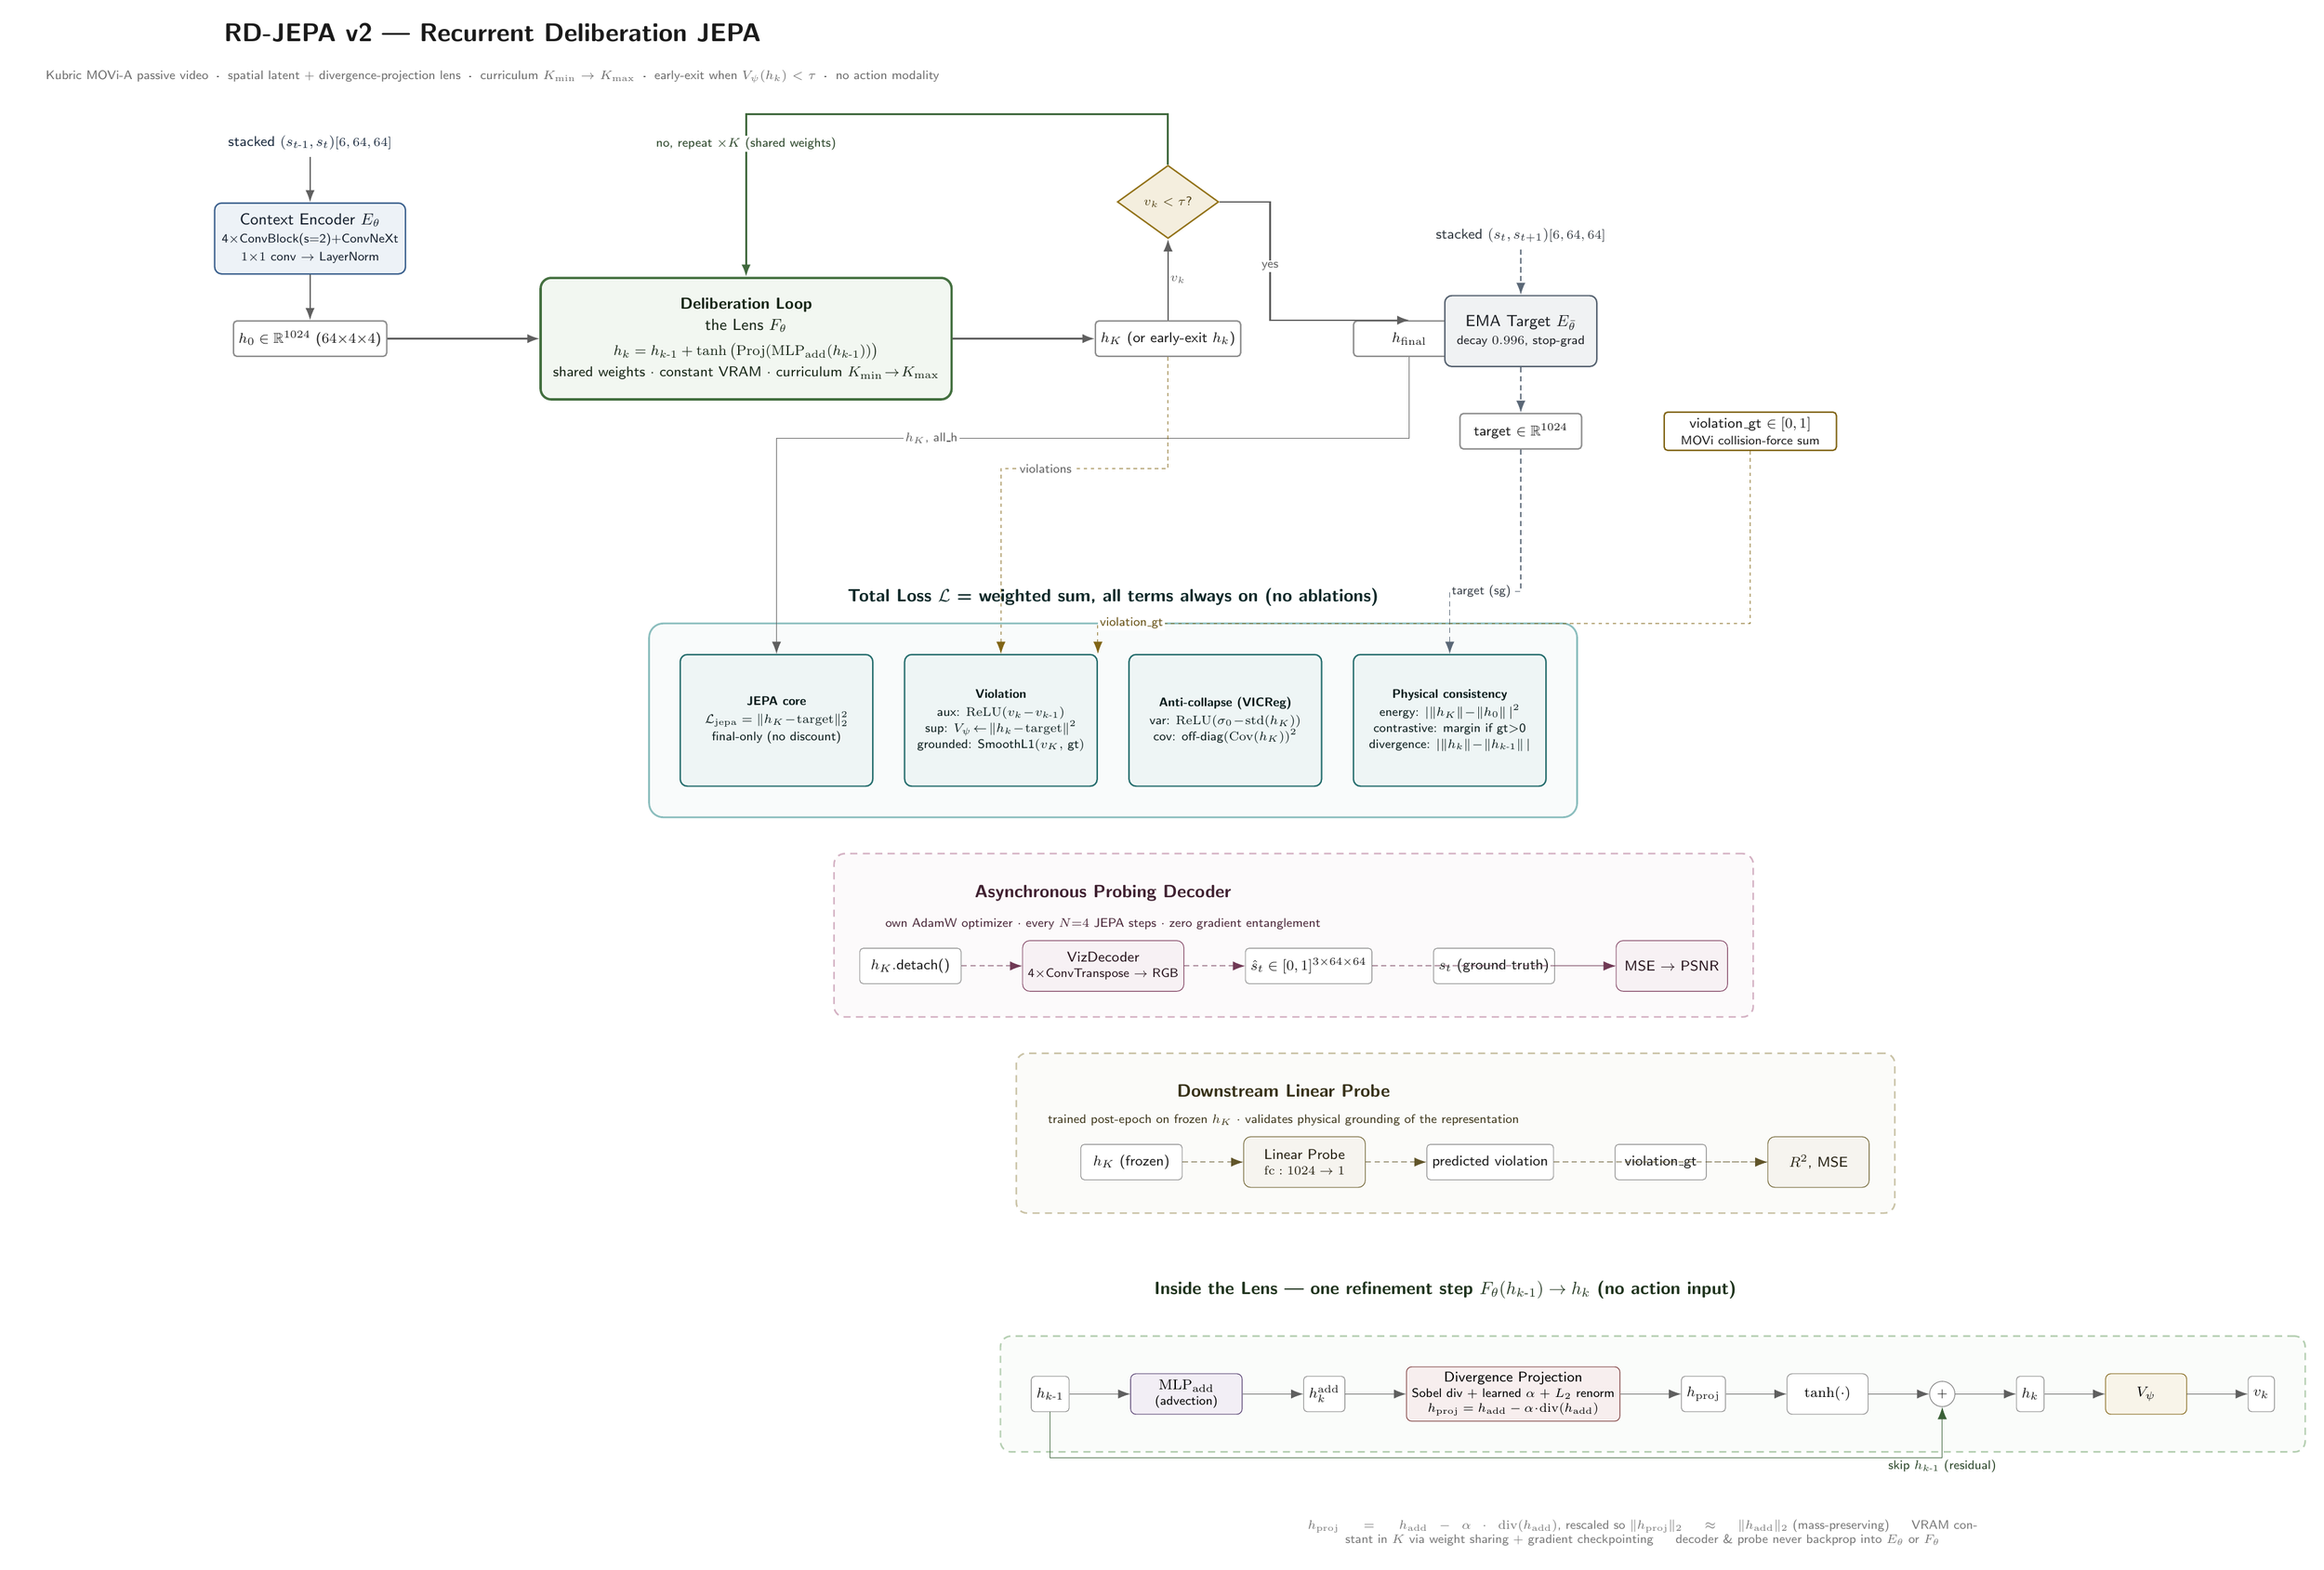
\begin{tikzpicture}[
  font=\sffamily\small,
  >={Latex[length=2.4mm]},
  thick,
  node distance=9mm and 12mm,
  enc/.style={draw=enc!80!black, fill=enc!10, rounded corners=4pt, align=center, inner sep=4pt, minimum width=32mm, minimum height=14mm, text=enc!25!black},
  lensblock/.style={draw=lens!75!black, line width=1.3pt, fill=lens!8, rounded corners=6pt, align=center, inner sep=7pt, minimum width=44mm, minimum height=24mm, text=lens!25!black},
  ema/.style={draw=target!80!black, fill=target!10, rounded corners=4pt, align=center, inner sep=4pt, minimum width=30mm, minimum height=14mm, text=target!25!black},
  los/.style={draw=loss!80!black, fill=loss!8, rounded corners=4pt, align=center, inner sep=3pt, minimum width=38mm, minimum height=26mm, text=loss!20!black, font=\sffamily\scriptsize},
  decbox/.style={draw=dec!80!black, fill=dec!8, rounded corners=4pt, align=center, inner sep=3pt, minimum height=10mm, font=\sffamily\footnotesize, text=dec!25!black},
  probebox/.style={draw=probe!80!black, fill=probe!8, rounded corners=4pt, align=center, inner sep=3pt, minimum height=10mm, font=\sffamily\footnotesize, text=probe!25!black},
  latent/.style={draw=ink!50, fill=white, rounded corners=2pt, align=center, inner sep=3pt, minimum height=7mm, font=\sffamily\footnotesize, text=ink},
  decision/.style={diamond, draw=vio!80!black, fill=vio!15, align=center, inner sep=2pt, font=\sffamily\scriptsize, text=vio!40!black, minimum width=20mm, minimum height=14mm},
  smallnode/.style={draw=add!70!black, fill=add!10, rounded corners=3pt, align=center, inner sep=3pt, minimum height=8mm, font=\sffamily\footnotesize},
  op/.style={circle, draw=ink!55, fill=white, inner sep=0pt, minimum size=5mm, font=\sffamily\scriptsize, text=ink},
  arr/.style={->, draw=ink!70},
  tarr/.style={->, draw=target!85!black, dash pattern=on 3pt off 2pt},
  garr/.style={->, draw=vio!70!black, dash pattern=on 2pt off 2pt},
  darr/.style={->, draw=dec!70!black, dash pattern=on 3pt off 2pt},
  parr/.style={->, draw=probe!70!black, dash pattern=on 3pt off 2pt},
  lab/.style={font=\sffamily\scriptsize, text=ink!70, inner sep=1pt, fill=white},
]

% ===================== TITLE ==============================================
\node[font=\sffamily\bfseries\Large, text=ink] (title) {RD-JEPA v2 — Recurrent Deliberation JEPA};
\node[font=\sffamily\scriptsize, text=ink!65, text width=185mm, align=center, below=3mm of title] (subtitle)
  {Kubric MOVi-A passive video \;·\; spatial latent + divergence-projection lens \;·\; curriculum $K_{\min}\!\to\!K_{\max}$ \;·\; early-exit when $V_\psi(h_k)\!<\!\tau$ \;·\; no action modality};

% ===================== MAIN PIPELINE =======================================
\node[font=\sffamily\footnotesize, text=enc!35!black, below=16mm of title, xshift=-36mm] (stp) {stacked $(s_{t\text{-}1},s_t)$\\[-1pt]\scriptsize $[6,64,64]$};
\node[enc, below=of stp] (encb) {Context Encoder $E_\theta$\\[-1pt]\scriptsize 4$\times$ConvBlock(s=2)+ConvNeXt\\[-1pt]\scriptsize $1{\times}1$ conv $\to$ LayerNorm};
\node[latent, minimum width=26mm, below=of encb] (h0) {$h_0\in\mathbb{R}^{1024}$ ($64{\times}4{\times}4$)};

\node[lensblock, right=30mm of h0] (lens)
  {\bfseries Deliberation Loop\\[1pt] the Lens $F_\theta$\\[3pt]
   \footnotesize $h_k = h_{k\text{-}1}+\tanh\big(\mathrm{Proj}(\mathrm{MLP}_{\mathrm{add}}(h_{k\text{-}1}))\big)$\\[1pt]
   \footnotesize shared weights $\cdot$ constant VRAM $\cdot$ curriculum $K_{\min}\!\to\!K_{\max}$};

\node[latent, minimum width=20mm, right=28mm of lens] (hK) {$h_K$ (or early-exit $h_k$)};
\node[decision, above=16mm of hK] (exit) {$v_k<\tau$?};
\node[latent, minimum width=22mm, right=22mm of hK] (hfinal) {$h_{\mathrm{final}}$};

\draw[arr] (stp) -- (encb);
\draw[arr] (encb) -- (h0);
\draw[arr] (h0) -- (lens);
\draw[arr] (lens) -- (hK);
\draw[arr] (hK.north) -- (exit.south) node[lab, midway, right] {$v_k$};
\draw[arr] (exit.east) -- ++(1.0,0) |- (hfinal.north) node[lab, pos=0.3, above] {yes};
\draw[arr, draw=lens!70!black, line width=1.1pt] (exit.north) -- ++(0,10mm) -| (lens.north)
  node[lab, pos=0.62, above, text=lens!45!black] {no, repeat $\times K$ (shared weights)};

% ===================== EMA TARGET + GROUNDED VIOLATION SIGNAL =============
\node[font=\sffamily\footnotesize, text=target!45!black, above=14mm of hfinal, xshift=22mm] (stp1) {stacked $(s_t,s_{t+1})$\\[-1pt]\scriptsize $[6,64,64]$};
\node[ema, below=of stp1] (emab) {EMA Target $E_{\bar\theta}$\\[-1pt]\scriptsize decay $0.996$, stop-grad};
\node[latent, minimum width=24mm, below=of emab] (target) {target $\in\mathbb{R}^{1024}$};
\draw[tarr] (stp1) -- (emab);
\draw[tarr] (emab) -- (target);

\node[latent, minimum width=34mm, right=16mm of target, draw=vio!70!black] (vgt) {violation\_gt $\in[0,1]$\\\scriptsize MOVi collision-force sum};

% ===================== LOSS (4 grouped panels) ==============================
\node[los, below=50mm of lens, xshift=6mm] (ljepa) {\bfseries JEPA core\\[2pt]\scriptsize $\mathcal{L}_{\mathrm{jepa}}=\|h_K\!-\!\mathrm{target}\|_2^2$\\[2pt]\scriptsize final-only (no discount)};
\node[los, right=6mm of ljepa] (lviol) {\bfseries Violation\\[2pt]\scriptsize aux: $\mathrm{ReLU}(v_k\!-\!v_{k\text{-}1})$\\[1pt]\scriptsize sup: $V_\psi\!\leftarrow\!\|h_k\!-\!\mathrm{target}\|^2$\\[1pt]\scriptsize grounded: SmoothL1$(v_K,$ gt$)$};
\node[los, right=6mm of lviol] (lcollapse) {\bfseries Anti-collapse (VICReg)\\[2pt]\scriptsize var: $\mathrm{ReLU}(\sigma_0\!-\!\mathrm{std}(h_K))$\\[1pt]\scriptsize cov: off-diag$(\mathrm{Cov}(h_K))^2$};
\node[los, right=6mm of lcollapse] (lphys) {\bfseries Physical consistency\\[2pt]\scriptsize energy: $|\|h_K\|\!-\!\|h_0\|\,|^2$\\[1pt]\scriptsize contrastive: margin if gt$>$0\\[1pt]\scriptsize divergence: $|\|h_k\|\!-\!\|h_{k\text{-}1}\|\,|$};

\begin{pgfonlayer}{background}
  \node[fit=(ljepa)(lviol)(lcollapse)(lphys), draw=loss!55, line width=1pt, fill=loss!3, inner sep=6mm, rounded corners=8pt] (lossgroup) {};
\end{pgfonlayer}
\node[font=\sffamily\bfseries, text=loss!30!black, above=2mm of lossgroup.north] {Total Loss $\mathcal{L}$ = weighted sum, all terms always on (no ablations)};

% all feeds travel through the CLEAR GAP above the loss group, then drop
% straight down into each panel's own top edge — never sideways through
% a neighbouring panel.
\draw[arr] (hfinal.south) -- ++(0,-16mm) -| (ljepa.north) node[lab, pos=0.4, right] {$h_K$, all\_h};
\draw[garr] (hK.south) -- ++(0,-22mm) -| (lviol.north) node[lab, pos=0.45, right] {violations};
\draw[tarr] (target.south) -- ++(0,-28mm) -| (lphys.north) node[lab, pos=0.5, right, text=target!50!black] {target (sg)};
\draw[garr] (vgt.south) -- ++(0,-34mm) -| (lviol.north east) node[lab, pos=0.5, right, text=vio!55!black] {violation\_gt};

% ===================== ASYNC DECODER BRANCH (auxiliary, no grad coupling) =
\node[font=\sffamily\bfseries, text=dec!40!black, below=12mm of lossgroup.south, xshift=-2mm] (dectitle) {Asynchronous Probing Decoder};
\node[font=\sffamily\scriptsize, text=dec!45!black, below=1mm of dectitle] (decsub) {own AdamW optimizer $\cdot$ every $N{=}4$ JEPA steps $\cdot$ zero gradient entanglement};
\node[latent, minimum width=20mm, below=8mm of dectitle, xshift=-38mm] (hkdet) {$h_K$.detach()};
\node[decbox, right=of hkdet, minimum width=26mm] (vizdec) {VizDecoder\\[-1pt]\scriptsize 4$\times$ConvTranspose $\to$ RGB};
\node[latent, minimum width=18mm, right=of vizdec] (predframe) {$\hat{s}_t\in[0,1]^{3\times64\times64}$};
\node[latent, minimum width=16mm, right=of predframe] (strue) {$s_t$ (ground truth)};
\node[decbox, right=of strue, minimum width=22mm] (decloss) {MSE $\to$ PSNR};
\draw[darr] (hkdet) -- (vizdec);
\draw[darr] (vizdec) -- (predframe);
\draw[darr] (predframe) -- (decloss);
\draw[darr] (strue) -- (decloss);
\begin{pgfonlayer}{background}
  \node[fit=(dectitle)(decsub)(hkdet)(vizdec)(predframe)(strue)(decloss), draw=dec!45, dash pattern=on 4pt off 3pt, line width=0.9pt, fill=dec!3, inner sep=5mm, rounded corners=6pt] (decgroup) {};
\end{pgfonlayer}

% ===================== LINEAR PROBE BRANCH (post-epoch, frozen model) =====
\node[font=\sffamily\bfseries, text=probe!40!black, below=12mm of decgroup.south, xshift=-2mm] (probetitle) {Downstream Linear Probe};
\node[font=\sffamily\scriptsize, text=probe!45!black, below=1mm of probetitle] (probesub) {trained post-epoch on frozen $h_K$ $\cdot$ validates physical grounding of the representation};
\node[latent, minimum width=20mm, below=8mm of probetitle, xshift=-30mm] (hkfrozen) {$h_K$ (frozen)};
\node[probebox, right=of hkfrozen, minimum width=24mm] (probemod) {Linear Probe\\[-1pt]\scriptsize $\mathrm{fc}: 1024\to1$};
\node[latent, minimum width=20mm, right=of probemod] (predviol) {predicted violation};
\node[latent, minimum width=18mm, right=of predviol] (gtviol) {violation\_gt};
\node[probebox, right=of gtviol, minimum width=20mm] (probemetric) {$R^2$, MSE};
\draw[parr] (hkfrozen) -- (probemod);
\draw[parr] (probemod) -- (predviol);
\draw[parr] (predviol) -- (probemetric);
\draw[parr] (gtviol) -- (probemetric);
\begin{pgfonlayer}{background}
  \node[fit=(probetitle)(probesub)(hkfrozen)(probemod)(predviol)(gtviol)(probemetric), draw=probe!45, dash pattern=on 4pt off 3pt, line width=0.9pt, fill=probe!3, inner sep=5mm, rounded corners=6pt] (probegroup) {};
\end{pgfonlayer}

% ===================== DETAIL INSET: one refinement step (self-contained) ==
\node[font=\sffamily\bfseries, text=lens!35!black, below=12mm of probegroup.south, xshift=-2mm] (insettitle) {Inside the Lens — one refinement step $F_\theta(h_{k\text{-}1})\to h_k$ (no action input)};

\node[latent, below=14mm of insettitle, xshift=-78mm] (i_hin) {$h_{k\text{-}1}$};
\node[smallnode, right=of i_hin, minimum width=22mm] (i_add) {$\mathrm{MLP}_{\mathrm{add}}$\\[-1pt]\scriptsize (advection)};
\node[latent, right=of i_add] (i_hadd) {$h^{\mathrm{add}}_k$};
\node[smallnode, draw=proj!70!black, fill=proj!10, right=of i_hadd, minimum width=34mm] (i_proj) {Divergence Projection\\[-1pt]\scriptsize Sobel div $+$ learned $\alpha$ $+$ $L_2$ renorm\\[-1pt]\scriptsize $h_{\mathrm{proj}}=h_{\mathrm{add}}-\alpha\!\cdot\!\mathrm{div}(h_{\mathrm{add}})$};
\node[latent, right=of i_proj] (i_hproj) {$h_{\mathrm{proj}}$};
\node[smallnode, draw=ink!50, fill=white, right=of i_hproj, minimum width=16mm] (i_tanh) {$\tanh(\cdot)$};
\node[op, right=of i_tanh] (i_res) {$+$};
\node[latent, right=of i_res] (i_hout) {$h_k$};
\node[smallnode, draw=vio!70!black, fill=vio!10, right=of i_hout, minimum width=16mm] (i_vio) {$V_\psi$};
\node[latent, right=of i_vio] (i_vout) {$v_k$};

\draw[arr] (i_hin) -- (i_add);
\draw[arr] (i_add) -- (i_hadd);
\draw[arr] (i_hadd) -- (i_proj);
\draw[arr] (i_proj) -- (i_hproj);
\draw[arr] (i_hproj) -- (i_tanh);
\draw[arr] (i_tanh) -- (i_res);
\draw[arr] (i_res) -- (i_hout);
\draw[arr] (i_hout) -- (i_vio);
\draw[arr] (i_vio) -- (i_vout);

% skip / residual: short local arc BELOW the row
\draw[arr, draw=lens!65!black] (i_hin.south) -- ++(0,-9mm) -| (i_res.south)
  node[lab, pos=0.5, below, text=lens!45!black] {skip $h_{k\text{-}1}$ (residual)};

\begin{pgfonlayer}{background}
  \node[fit=(i_hin)(i_add)(i_hadd)(i_proj)(i_hproj)(i_tanh)(i_res)(i_hout)(i_vio)(i_vout),
        draw=lens!45, dash pattern=on 4pt off 3pt, line width=0.9pt, fill=lens!3,
        inner sep=6mm, rounded corners=6pt] (insetgroup) {};
\end{pgfonlayer}

% ===================== FOOTER ================================================
\node[font=\sffamily\scriptsize, text=ink!60, text width=185mm, align=center, below=12mm of insetgroup.south, xshift=-2mm]
  {$h_{\mathrm{proj}} = h_{\mathrm{add}} - \alpha\cdot\mathrm{div}(h_{\mathrm{add}})$, rescaled so $\|h_{\mathrm{proj}}\|_2\!\approx\!\|h_{\mathrm{add}}\|_2$ (mass-preserving) $\quad$
   VRAM constant in $K$ via weight sharing + gradient checkpointing $\quad$ decoder \& probe never backprop into $E_\theta$ or $F_\theta$};

\end{tikzpicture}
\end{document}
